\documentclass[11pt]{article}
\usepackage[sc]{mathpazo} %Like Palatino with extensive math support
\usepackage{fullpage}
\usepackage[authoryear,sectionbib,sort]{natbib}
\linespread{1.7}
\usepackage[utf8]{inputenc}
\usepackage{lineno}
\usepackage{titlesec}

\usepackage{graphicx,float}
% for setting up equations
\usepackage{amsmath}

\titleformat{\section}[block]{\Large\bfseries\filcenter}{\thesection}{1em}{}
\titleformat{\subsection}[block]{\Large\itshape\filcenter}{\thesubsection}{1em}{}
\titleformat{\subsubsection}[block]{\large\itshape}{\thesubsubsection}{1em}{}
\titleformat{\paragraph}[runin]{\itshape}{\theparagraph}{1em}{}[. ]\renewcommand{\refname}{Literature Cited}

%%%%%%%%%%%%%%%%%%%%%
% Line numbering
%%%%%%%%%%%%%%%%%%%%%
%
% Please use line numbering with your initial submission and
% subsequent revisions. After acceptance, please turn line numbering
% off by adding percent signs to the lines %\usepackage{lineno} and
% to %\linenumbers{} and %\modulolinenumbers[3] below.
%
% To avoid line numbering being thrown off around math environments,
% the math environments have to be wrapped using
% \begin{linenomath*} and \end{linenomath*}
%
% (Thanks to Vlastimil Krivan for pointing this out to us!)

\title{Increasing prevalence of plant-fungal symbiosis over 195 years of climate change}

% This version of the LaTeX template was last updated on
% September 28, 2022.

%%%%%%%%%%%%%%%%%%%%%
% Authorship
%%%%%%%%%%%%%%%%%%%%%
% Please remove authorship information while your paper is under review,
% unless you wish to waive your anonymity under double-blind review. You
% will need to add this information back in to your final files after
% acceptance.

\author{Joshua C. Fowler$^{1,\ast}$ \\
	Tom E. X. Miller$^{1}$}
\date{}

\begin{document}
	
	\maketitle
	
	\noindent{} 1. Rice University, Department of BioSciences, Houston, Texas 77006;


	\noindent{} $\ast$ Corresponding author; e-mail: jcf3@rice.edu.
	
	\bigskip
	
	\textit{Manuscript elements}: Figure~1, figure~2, table~1, appendix~A (for print; including figure~A1, figure~A2, and table~A1), supplemental PDF. Figure~2 is to print in color.
	
	\bigskip
	
	\textit{Keywords}: .
	
	\bigskip
	
	\textit{Manuscript type}: Article. %Or note, natural history miscellany note, comment, reply, invited symposium, featured topic, or historical perspective.
	
	\bigskip
	
	\noindent{\footnotesize Prepared using the suggested \LaTeX{} template for \textit{Am.\ Nat.}}
	
	%\linenumbers{}
	%\modulolinenumbers[3]
	
	\newpage{}
	
	\section*{Abstract}
Climate change has altered species’ phenologies, has triggered changes in traits, and has led to shifts in abundance and distributions. 
Yet, we still know little about how biotic interactions alter these environmental responses over long time scales across spatially heterogenous changes in climate. 
Most species host beneficial microbial symbionts, which may provide resilience to changes in the environment, but at the same time increasing stress may lead these symbioses to breakdown. 
Microbes can be preserved within the dried plant tissue of herbarium specimens presenting an opportunity to quantify changes across broad temporal and spatial scales. 
Epichloë fungal endophytes are seed-transmitted symbionts of cool-season grasses which can provide drought tolerance to their hosts. 
 We ask how endophyte prevalence has responded to climate change. 
 Specifically, we took samples of seeds from herbarium specimens of three grass host species collected over the last two centuries, quantified the presence or absence of fungal endophytes within the seeds with microscopy, and evaluated spatial and temporal trends in prevalence using spatial modeling.
 We found strong evidence that fungal endophyte prevalence has increased over the last two centuries across the three host species from 25\% prevalence to 75\% prevalence on average.
We also found that observed changed in annual  and seasonal climate drivers were associated with temporal trends in endophyte prevalence. 
In particular, changes in prevalence within each species corresponded to climate drivers during its peak growing season. 
Thus we provide novel evidence for adaptive biotic responses to ongoing climate change.


	
	\newpage{}
	
	\section*{Introduction}
	
	% The journal does not have numbered sections in the main portion of
	% articles. Please refrain from using section references (à la
	% section~\ref{section:CountingOwlEggs}), and refer to sections by name
	% (e.g. section ``Counting Owl Eggs'').
Predicting how species' interactions will be altered by ongoing climate change is a major goal of basic ecological research and conservation management. 
Spatially heterogeneous changes in the environment have led species to move, adapt, or face extinction \citep{IPCC2012managing}. 
Species' responses are likely mediated by the numerous interspecific interactions in which they engage. 
Yet for most species, empirically evaluating the role that biotic interactions can play in facilitating or hindering adaption to changing environmental conditions has been limited by a lack of data at adequate spatial and temporal scales \cite{gilman2010framework}.

Natural history collections, which were originally collected to study and preserve taxonomic diversity, present an exciting opportunity to explore long-term changes in ecological interactions across broad spatial scales \citep{meineke2018unrealized}. 
Natural history collections, built and maintained by the efforts of thousands of scientists, are invaluable time machines. 
These collections primarily comprise physical specimens of organisms  along with information about the time and place of their collection. 
These specimens are samples preserving physical legacies of ecological dynamics and species' interactions from dynamically changing environments across time and space.
Recent works using plant collections have documented changes in phenology \citep{willis2017old, park2019herbarium,  berg2019examination}, as well as pollination \citep{pauw2011reconstruction, duan2019century}, and changes in antagonistic interactions such as herbivory \citep{meineke2019herbarium}, but to date, focus has been lacking on long-term changes in a particularly common type of biotic interaction, microbial symbioses. 

Microbes are hosted by all organisms with documented effects on their hosts' survival, growth and reproduction \cite{rodriguez2009fungal,mcfall2013animals}.
Many microbial symbionts act as mutualists, engaging in reciprocally beneficial interactions with their hosts. 
These mutualisms play an important role in limiting the consequences of environmental stress. 
For example, bacterial symbionts of insects, such as \emph{Wolbachia}, can improve their hosts' thermal tolerance \citep{truitt2019wolbachia, renoz2019evolutionary}. Similarly, arbuscular mycorrhizal fungi, documented in 70-90\% of families of land plants \citep{parniske2008arbuscular}, allow their hosts to persist through drought conditions by improving water and nutrient uptake \citep{cheng2021elucidating}.
At the same time, changes in the mean and variance of environmental conditions may disrupt mutualisms by changing the costs and benefits of the interaction for each partner, leading to the extinction of one or both partner species \citep{aslan2013mutualism}. 
Coral bleaching, the loss of symbiotic algae due to temperature stress \citep{sully2019global} is perhaps the best known example, but this phenomenon is not unique to corals.
Lichens exposed to elevated temperatures experienced loss of photosynthetic function along with changes in the community composition of their algal symbionts \citep{meyer2022climate}.
Whether symbiotic mutualisms breakdown or promote resilience under climate change is unclear, but likely depends on the intimacy and specialization of the interaction, as well as the physiological tolerances of the mutualists \citep{toby2010mutualisms, warren2014mutualism, rafferty2015phenological}. 
Given that climate change is spatially heterogenous, the rate of change may have a strong influence on when and where we can expect facilitation or disruption of mutualism. 

Early research on \emph{Epichloë} fungal endophytes, specialized symbionts of cool-season grasses, used herbarium specimens to describe the broad taxonomic diversity of hosts \citep{white1985endophyte}. 
These facultative symbionts, which have been documented in $\sim 30$\% of cool-season grasses \citep{leuchtmann1992systematics}, are transmitted vertically from maternal plants to offspring through the grasses' seeds.
Vertical transmission creates a feedback between the fitness of host and symbiont \citep{fine1975vectors, douglas1998host, rudgers2009fungus}. 
Over time, endophytes that act as mutualists for their hosts should rise in prevalence within a population. 
\emph{Epichloë} are known to improve drought tolerance for their hosts \citep{afkhami2014mutualist}, and are expected to reach high prevalence where these fitness benefits are most important.
Previous survey studies have documented large-scale spatial patterns in  endophyte prevalence structured by environmental gradients \citep{granath2007variation,bazely2007broad, afkhami2012fungal,sneck2017variation}.
We predicted that prevalence should also track temporal changes in environmental drivers, but testing this has been impossible with surveys limited to a few years, and to the spatial extent reachable during a single growing season. 
Becauses the fungi are seed-transmitted, they are conveniently preserved along with their host plants on herbarium sheets, creating the opportunity to examine the response of the symbiosis to historical climate change.

In this study, we took advantage of the spatial and temporal sampling within herbaria to assess for the first time whether grass-fungal endophyte symbioses have responded adaptively to climate change. In particular, we (i) quantified the spatial and temporal change in endophyte prevalence across host ranges over the last two centuries, and (ii) identified climate drivers that can explain the magnitude of these responses.
	
\section*{Methods}
        \subsection*{Focal host species}
We focused on three endophyte hosts, \emph{Agrostis hyemalis}, \emph{Agrostis perennans}, and \emph{Elymus virginicus}.
These grass species, which are all cool-season (C3) grasses, are commonly represented in natural history collections with broad distributions covering the Eastern United States.
\emph{A. hyemalis} is a small short-lived perennial species that germinated in the spring and typically blooms between March and July.
\emph{A. perennans} of similar stature but blooms in late Summer and early Autumn. 
This species is relatively more  sparsely distributed, tending to be found in shadier and more moist habitats while \emph{A. hyemalis} is often found in open and recently disturbed ground. 
Both\emph{Agrostis} species are recorded from throughout the Eastern US, but \emph{A. perennans} has a slighty more northern distribution, whereas \emph{A. hyemalis} is found rarely as far north as Canada and is listed as a rare plant in Minnesota.
\emph{E. virginicus} is a larger and relatively longer-lived  species that is more broadly distributed that the \emph{Agrostis} species. 
It begins flowering as early as March or April but continues throughout the Summer.

		\subsection*{Herbarium surveys}
We collected 5-10 seeds per specimen during visits to natural history collections between 2019 and 2022 (See Table A1 for a summary of collections) . 
Grasses are commonly identified and collected based on the presence of their reproductive structures which ensured that specimens we examined contained seeds. 
Our sampling plan was designed to minimize damage to these specimens.

\begin{figure}[H]
	\centering
	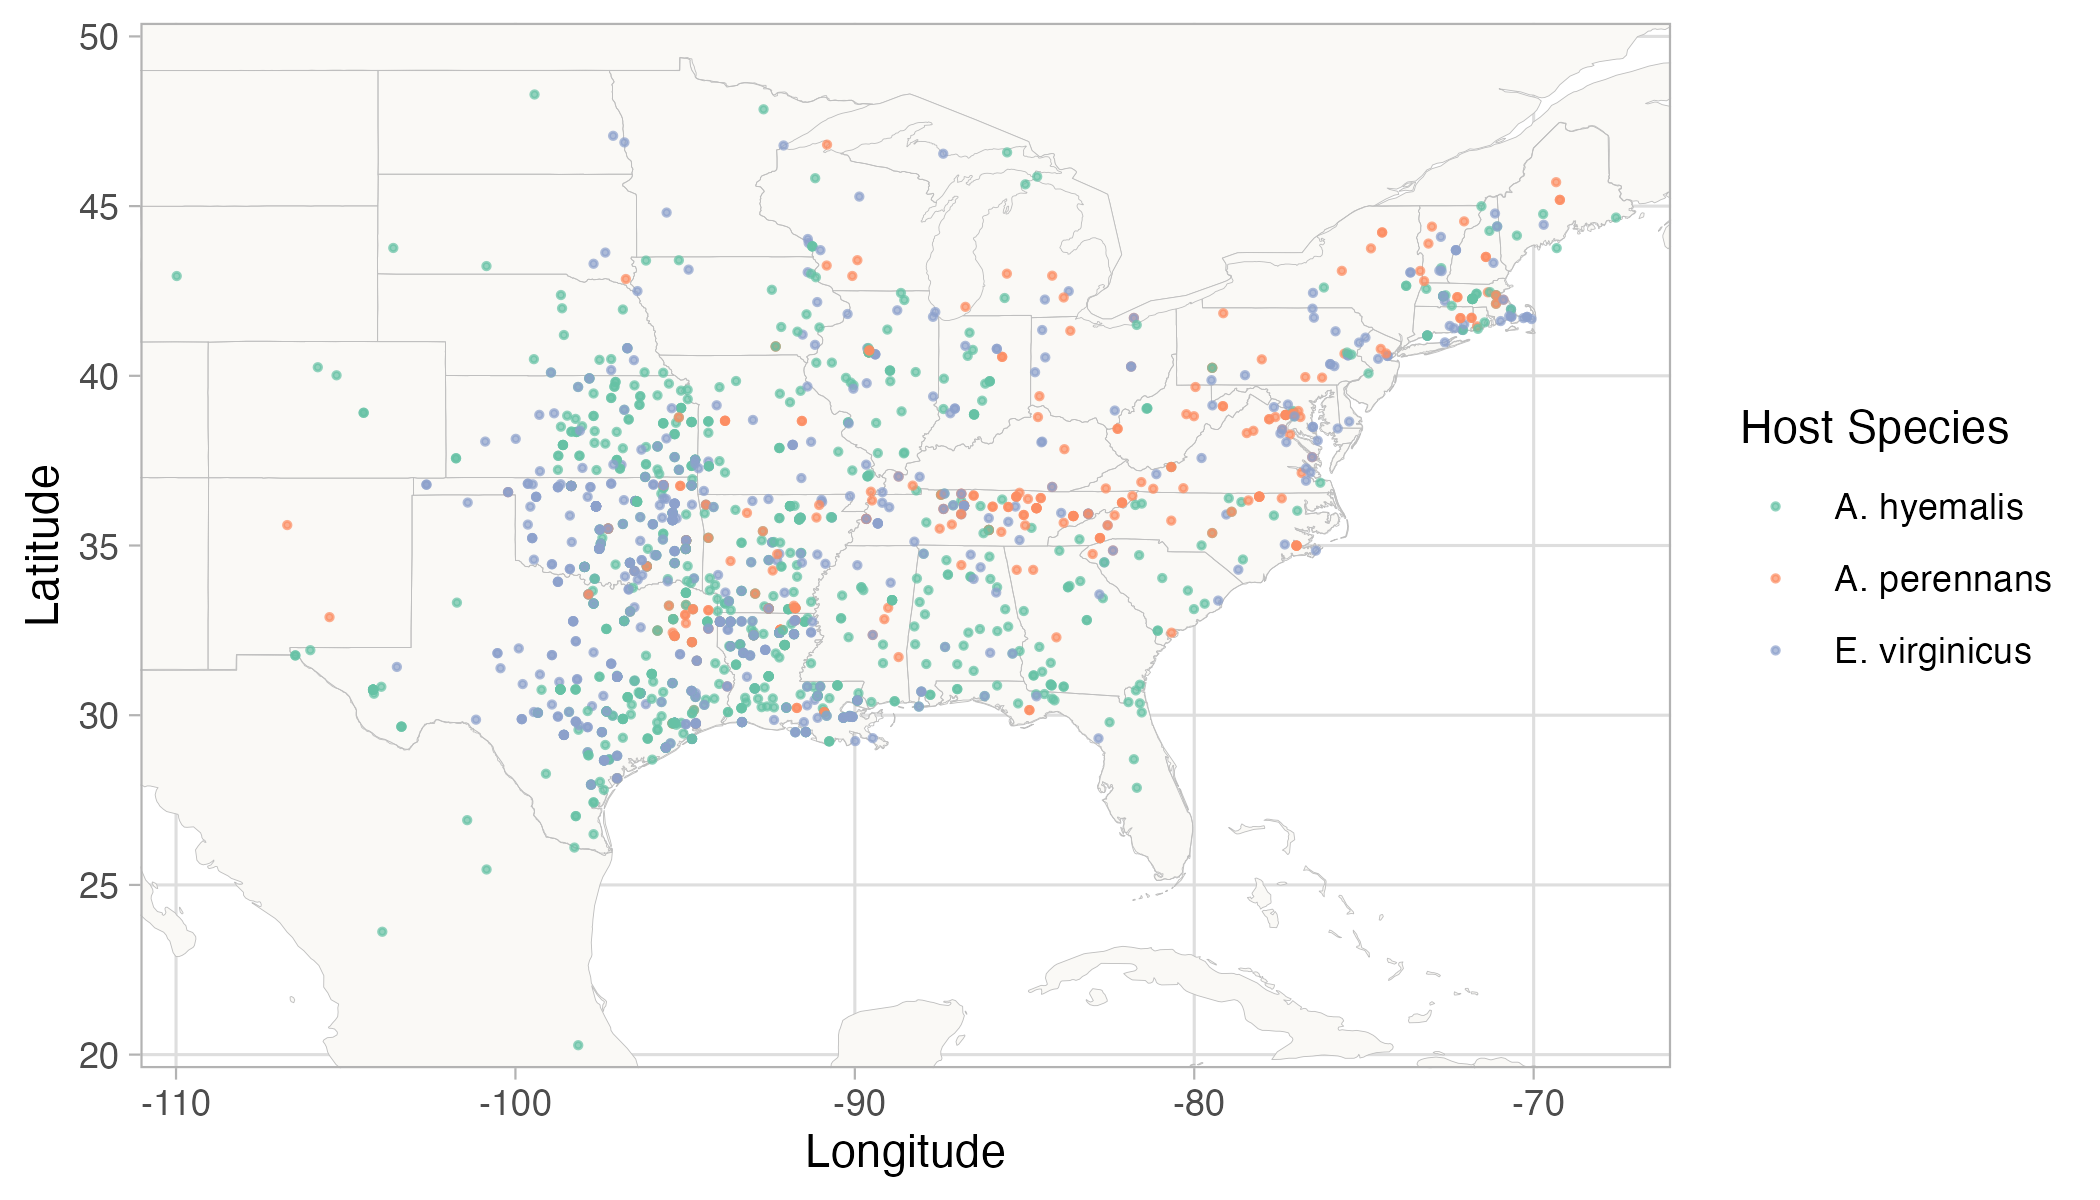
\includegraphics[width = \linewidth]{collections_map.png}
	\caption{\textbf{Collection locations of herbarium specimens sampled for endopnhyte presence absence}. Color designates host species ( \emph{A. hyemalis} (green), \emph{A. perennans} (orange), \emph{E. virginicus} (purple))}
\end{figure}


After collecting seeds, we quantified the presence or absence of \emph{Epichloë} fungal hyphae, which grow intercellularly, using microscopy. We first softened seeds with a 10\% NaOH solution, then stained the seeds with aniline blue dye and squashed them under a microscope cover slip. 
We examined the squashed seeds for the presence of fungal hyphae at 100X magnification \cite{bacon2018stains}.
We designated each specimen as symbiotic or non-symbiotic, a binary response variable, based on the presence of endophytes within any of the scored seeds for that specimen. 
In some cases, the tissues examined during microscopy came from flowers or otherwise non-viable seeds, which were excluded from the seed counts for that specimen.
To capture uncertainty in the identification process, we recorded both a "liberal" and a "conservative" endophyte status for each plant.  
When we identified potential endophytes with unusual morphology, low uptake of stain, or a small amount of fungal hyphae across the scored seeds, we recorded a positive liberal status (more likely to be a true endophyte) and a negative conservative status (less likely to be a true endophyte). 
$89$\% of scored plants had matching liberal and conservative endophyte statuses, reflecting high confidence in the endophyte identification.
The following analyses presented in the main text used the liberal statuses, but we repeated all analyses with the conservative statuses which yielded qualitatively similar results (Appendix). 

We excluded specimens that did not include information about the collection location and date from our sampling efforts.
In total, we quantified endophyte symbiosis for $971$ \emph{A. hyemalis}, $302$ \emph{A. perennans}, and $605$ \emph{E. virginicus} specimens spanning the years $1824$ to $2019$.
Each specimen was assigned a collection location based on geographic information recorded at the time of collection using the ggmap package in R \citep{kahle2019package}. 
Collections were georeferenced to the nearest county centroid, or nearest municipality when that information was available. For a few of the oldest specimens, only information at the state level was available, and so we used the state centoid (Fig. 1; Fig A1).


\subsection*{Assessing spatial and temporal changes in endophyte prevalence}
To quantify spatial and temporal trends in endophyte prevalence, we modelled endophyte presence/absence ($P$) as a Bernoulli distribution for specimen $i$ of host species $h$.

\begin{subequations}
		\label{eq:trends}
		\begin{align}
		P_{i,h} \sim Bernoulli(\hat{P_{h}}) \\
			logit(\hat{P}_{h}) = \beta_{0,h} + 
		\beta_{1,h}*year_{i} + \\
		\beta_{2,h}*year_{i} *lat_{i} + 
		\beta_{3,h}*year_{i} *lon_{i} + 
		\beta_{4,h}*year_{i} *lat_{i}*lon_{i} +\\
		\chi + \omega + \phi
		\end{align}
\end{subequations}

The expected endophyte prevalence, $\hat{P}$, was modelled with intercepts specific to each host species ($\beta_{0}$), slopes for changes over time ($\beta_{1}$) as well as the interaction between time and the specimen's latitude and longitude ($\beta_{2}$, $\beta_{3}$, and $\beta_{4}$). 
We accounted for potential biases introduced during the process of collecting specimens as well as in scoring ability by including random effects specific to each collector $\chi$ and to each scorer $\omega$.
To quantify spatial patterns in prevalence, we included a spatially-dependent random intercept, $\phi$, and fit the model using integrated nested Laplace approximation, an approximate Bayesian method implemented in the rINLA package \citep{lindgren2015bayesian}. 
This method allowed us to model spatial dependency between data points as a continuous process with stochastic partial differential equations (SPDE) that depend on a covariance matrix according to the proximity of each collection location \citep{lindgren2011explicit,bakka2018spatial}. 
The covariance matrix is approximated using a Matérn covariance function, with each data point assigned a location according to the nodes of a mesh of non-overlapping triangles across our study area (Fig A2).
We fit the model with vague priors, and compared models with different sizes of mesh, which had little effect on the resulting model estimates.
We assessed model fit with graphical postterior predictive checks (Fig. A3, Fig. A4).

We used data on endophyte prevalence from  contemporary surveys of \emph{A. hyemalis} as test data to evaluate model fit. 
During these surveys, which took place between 2015 and 2020, we collected seeds from living plants from 43 populations across a portion of the species' range and then quantified endophyte status with staining microscopy as described for the herbarium surveys (Fig S2).
We compared the model's prediction for these locations to the endophyte status of randomly sampled plants from each surveyed location, mimicing the process of collecting a single herbarium specimen from the population.
The model performed adequately (training data: AUC = 0.77; test data: AUC = 081; Fig. A4). 

		\subsection*{Assessing the role of climate drivers}
To assess how the rate of climate change may have driven changes in endophyte prevalence, we calculated the change in climate between recent (1990 to 2020) and historic (1895 to 1925) periods.
We first downloaded monthly temperature and precipitation rasters from the PRISM climate group \citep{daly2013prism} covering the time period between 1895 and 2020 using the 'prism' R package \citep{Rprism2015}. 
Prism provides reconstructions of historic climate variables across the United States by spatially-interpolating weather station data \citep{diLuzio2008constructing}. 
We calculated 30-year climate normals for annual and seasonal mean temperature and cumulative precipitation for the recent and historic periods.
We used three four-month seasons within the year (Spring: January, February, March, April; Summer: May; June, July, August; Autumn: September, October, November, December). 
We additionally calculated the coefficient of variation of each climate driver during each period.
We then took the difference between recent and historic periods for the mean and coefficient of each climate driver (Fig. A5).
Because initial analyses indicated a high degree of collinearity between seasonal and annual changes in temperature, we used annual temperature only, along with annual and seasonal precipitation, in the subsequent analysis.

We then evaluated how predicted changes in endophyte prevalence correlated with changes in thee environment at an evenly spaced grid of points across the study area. 
Because regions varied in their predicted starting endophyte prevalence, we calculated the relative change in endophyte prevalence between 1925 and 2020. 
This time period connects the predicted change in prevalence with the endpoints of the available climate record.
We then calculated the Pearson correlation coefficient between the relative change in endophyte prevalence and each climate driver. 

%We evaluated how predicted changes in endophyte prevalence ($\Delta{P}$) correlated with %changes in seasonal climate at a grid of points across the study area using linear regression.

%\begin{subequations}
	%\label{eq:climate}
	%\begin{align}
		%\Delta{P} \sim Normal(\mu, \sigma)\\
		%\mu = \beta_{0} + \alpha_{1}*\Delta{Precip_{spring}} + %\alpha_{2}*\Delta{Precip_{summer}} + \alpha_{3}*\Delta{Precip_{autumn} }+ \\ %\alpha_{4}*\Delta{Temp_{spring}} + \alpha_{5}*\Delta{Temp_{summer}}  + %\alpha_{6}*\Delta{Temp_{autumn}} 
%	\end{align}
%\end{subequations}

 %The change in prevalence is determined by an intercept $\beta_{0}$ slopes specific to the seasonal %changes in preciptation ($\alpha_{1}$, $\alpha_{2}$, and $\alpha_{3}$) and in mean %temperature ($\alpha_{4}$, $\alpha_{5}$, and $\alpha_{6}$).
 %We fit models for each host species separately with rINLA using default vague priors.
		
\section*{Results}

\subsection*{Temporal and spatial trends}

We found that endophyte prevalence increased within the examined specimens over the last two centuries for all three host species (Fig. 2). 
On average, \emph{A. hyemalis} and \emph{E. virginicus} both increased from ~30 \% to over 50\% prevalence across the study region, and \emph{A. perennans} increased from ~ 15\% to over 70\% prevalence.
Rerunning the analysis excluding specimens collected before 1900 when samples are much sparser (Fig. 2A), lead to qualitatively similar predictions, and so we continued analyses with the full dataset. 

\begin{figure}[H]
	\centering
	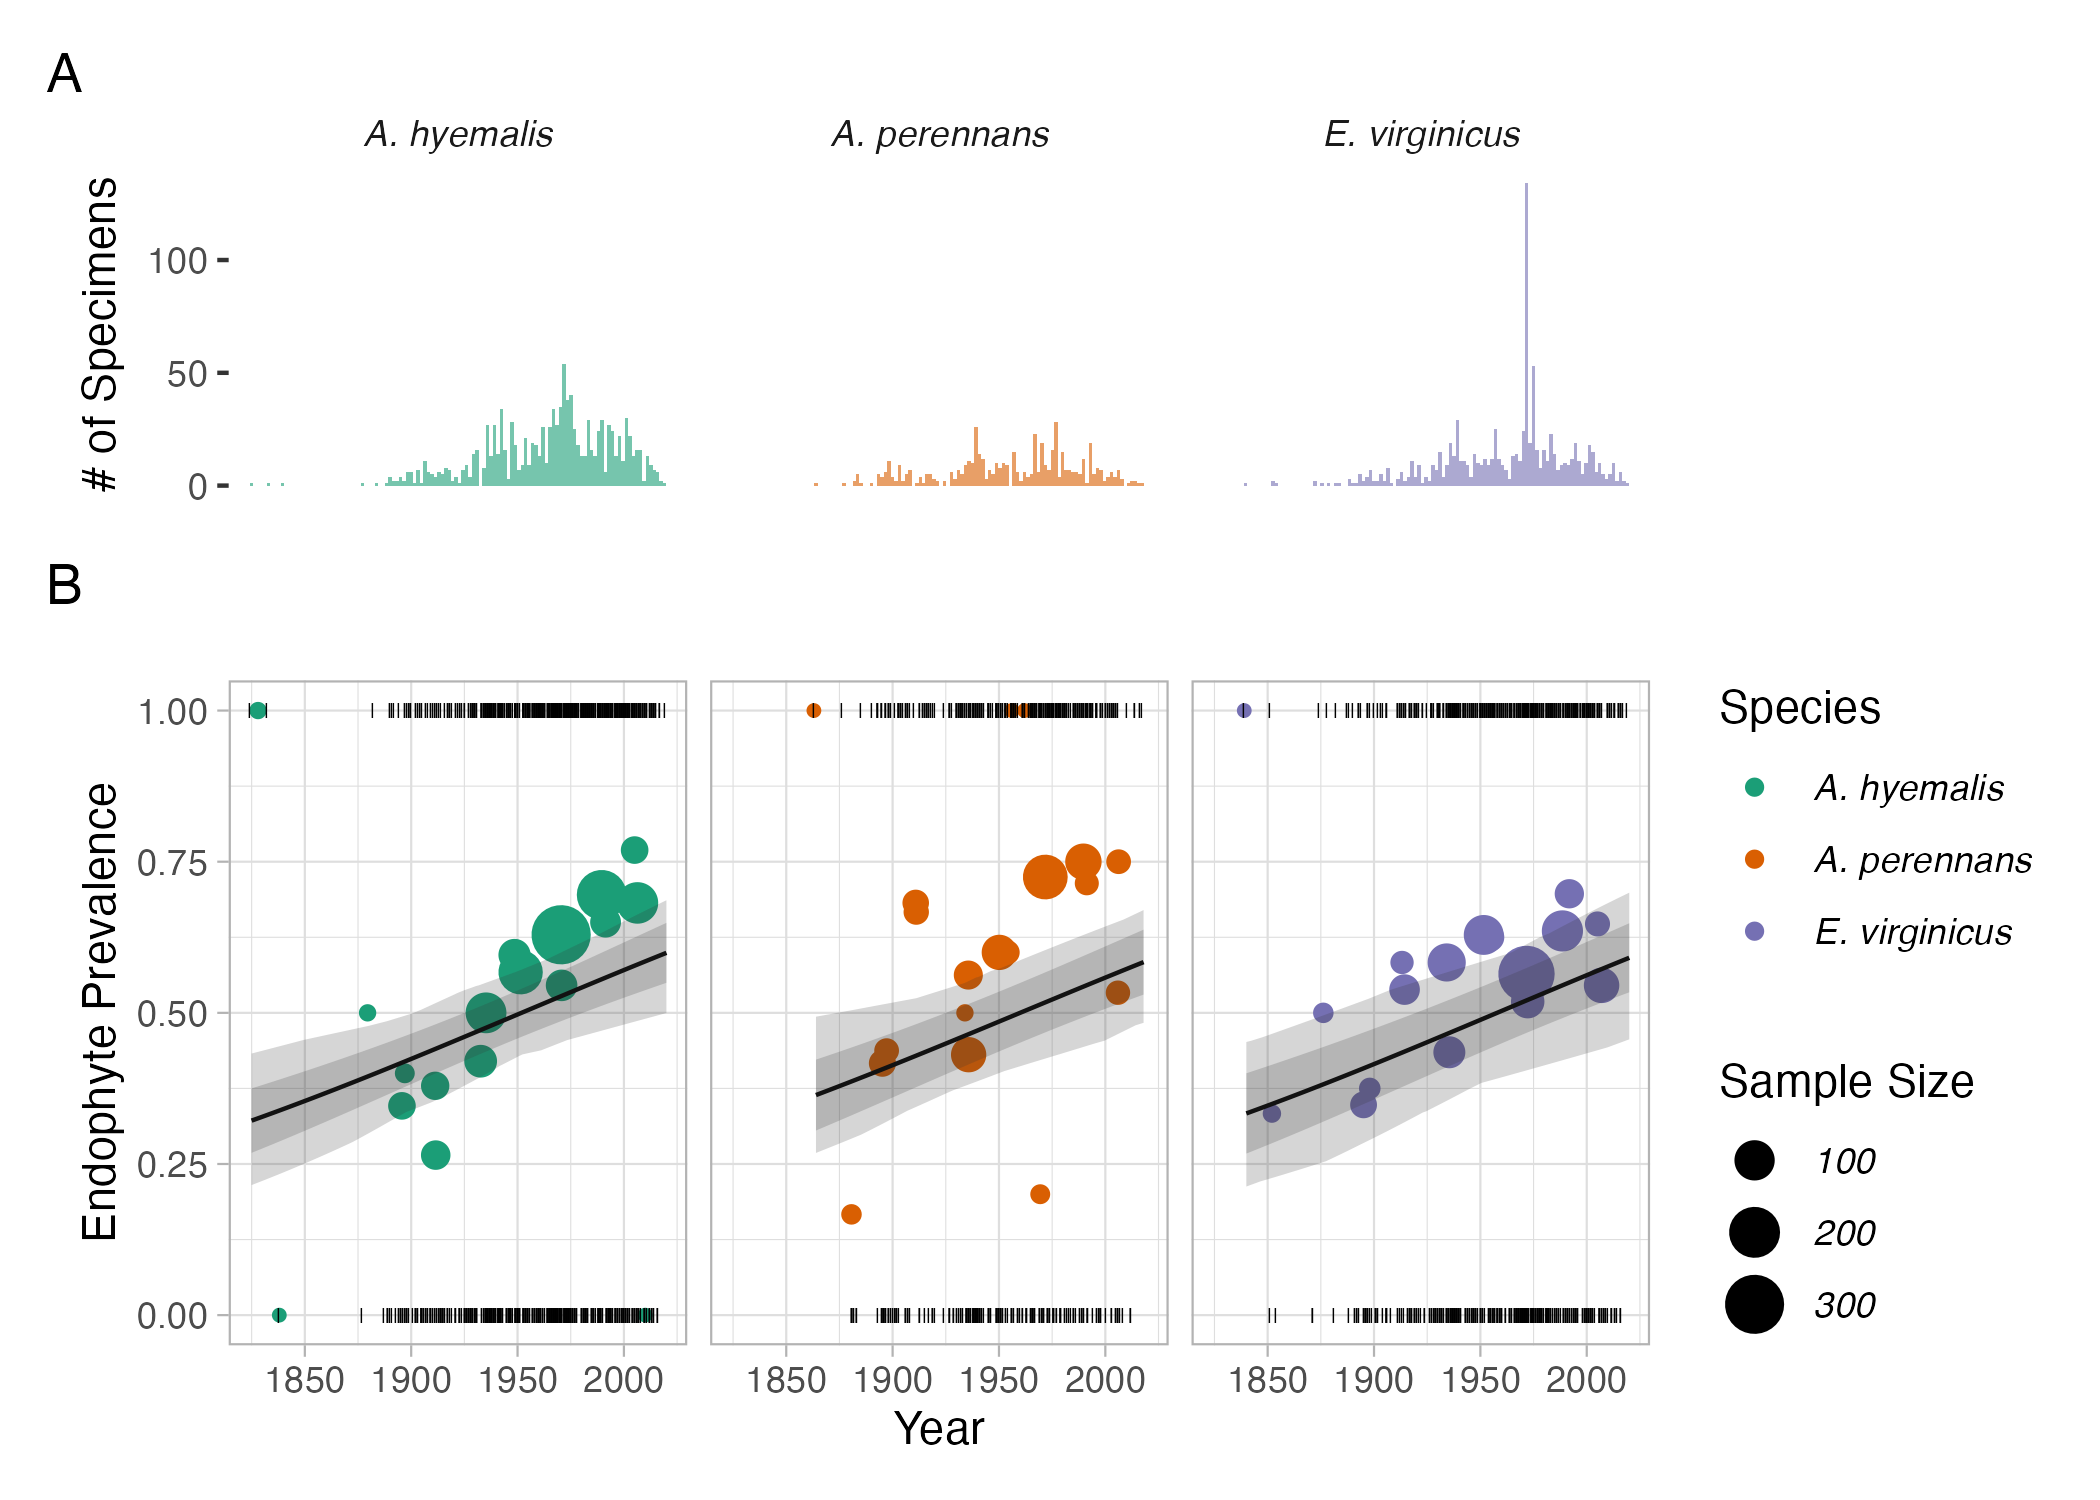
\includegraphics[width = \linewidth]{year_plot.png}
	\caption{\textbf{Temporal trends in endophyte prevalence.} (A) Histograms show the frequency of collection through time for each host species. (B) Colored points are binned means of the observed endophyte presence/absence data (black dashes). Colors represent each host species and point size is determined by the number of specimens. Lines show predicted mean endophyte prevalence over the study period at low (dotted) high (solid) latitudes and along with 95\% CI bands.}
\end{figure}

Across space, there were clear trends in endophyte prevalence which varied between species (Fig. 3). 
For example, \emph{Elymus virginicus}, had higher prevalence in the northern and eastern portions of it's range. 
In contrast, \emph{Agrostis hyemalis} had highest prevalence towards the center of its range with regions of low prevalence towards the north east and towards its western range edge.
Our model revealed that while there was an overall increase in endophyte prevalence, these changes varied across the host species' ranges.
In some regions, \emph{A. perennans} experienced increases in percent prevalence by as much as 35 percentage points between 1920 and 2020, while \emph{A. hyemalis} and \emph{E. virginicus} experienced increases up to around 15 percentage points. 
In other regions, there were smaller increases of only five percentage points for \emph{E. virginicus} and fifteen percentage points for \emph{A. perennans}. 
Notably, the western range edge of \emph{A. hyemalis} did not experience an increase in endophyte prevalence. 
Collections are sparser to the west as the species reaches its range limit, but the collected specimens were exclusively symbiont-free. (Fig. A1). 

\begin{figure}[H]
	\label{fig:prevalence_map}
	\centering
	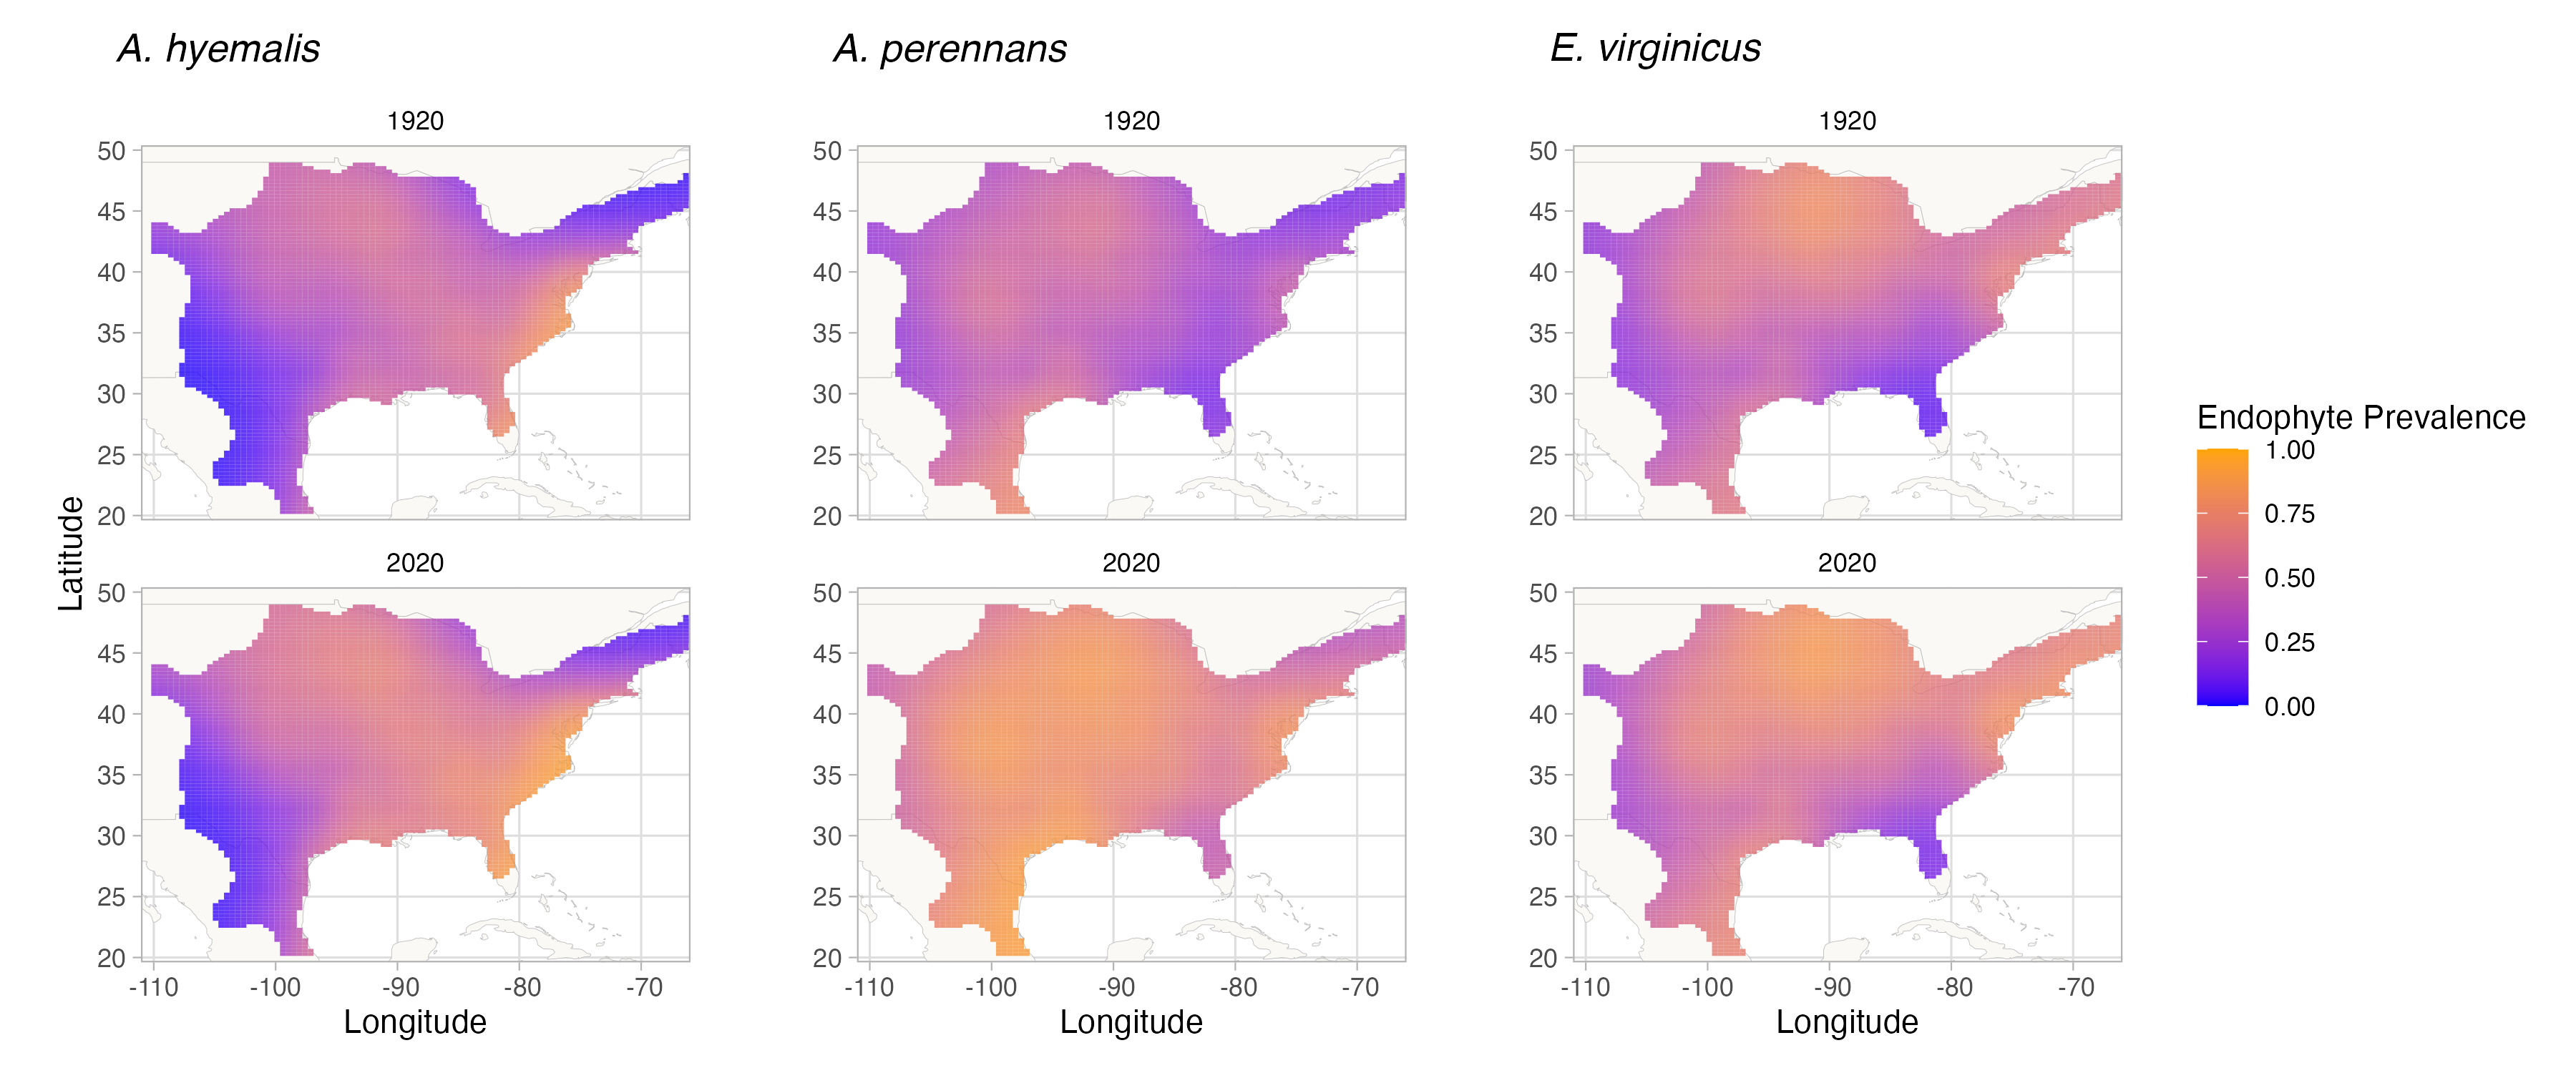
\includegraphics[width = \linewidth]{prevalence_map.png}
	\caption{\textbf{Mean predicted endophyte prevalence for each host species (columns) in 1920 (top row) and 2020 (bottom row)}. Color indicates mean predicted rate of endophyte prevalence.}
\end{figure}


\subsection*{The role of climate drivers}
We found that the trends in endophyte prevalence were strongly associated with seasonal climate change drivers (Fig. 4). 
For the majority of the study region, the climate has become wetter and cooler over the last century (Fig. A5), a consequence of regional variation in global climate change. 
Within the study region, spatially heterogeneous environmental changese were predictive of changes in endophyte prevalence in line with differences in species' reproductive timing. 
For example, relative change in endophyte prevalence within \emph{E. virginicus} were most associated with declines in Summer precipitation  (a negative correlation in Fig. 4) as well as with increases in the year-to-year variability of summer precipitation (a positive correlation in Fig. 4).
These associations are in line with expectations that endophyte symbiosis provides drought tolerance to their hosts, particularly during \emph{E. virginicus}'s summer growing season. 
For \emph{A. perennans}, which typically flowers in the late Summer and Autumn, increases in autumn precipitation along with increases in variability in annual precipitation, were strongly assocated with increasing endophyte prevalence.  
While this result is contrary to the expectation that endophyte provide drought tolerance, this species typically is associated with wetter microhabitats, and it also suggests a role for endophytes to play in buffering the negative consequences of demographic variability \citep{lewontin_population_1969}.  
For \emph{A. hyemalis}, which flowers in the Spring, changes in endophyte prevalence were more weakly associated with seasonal changes in climate drivers than for the other two species.
It was, however, the only species' for which greater increases in endophyte prevalence were associated with regions that experienced increases in average annual temperatures.

\begin{figure}[H]
	\centering
	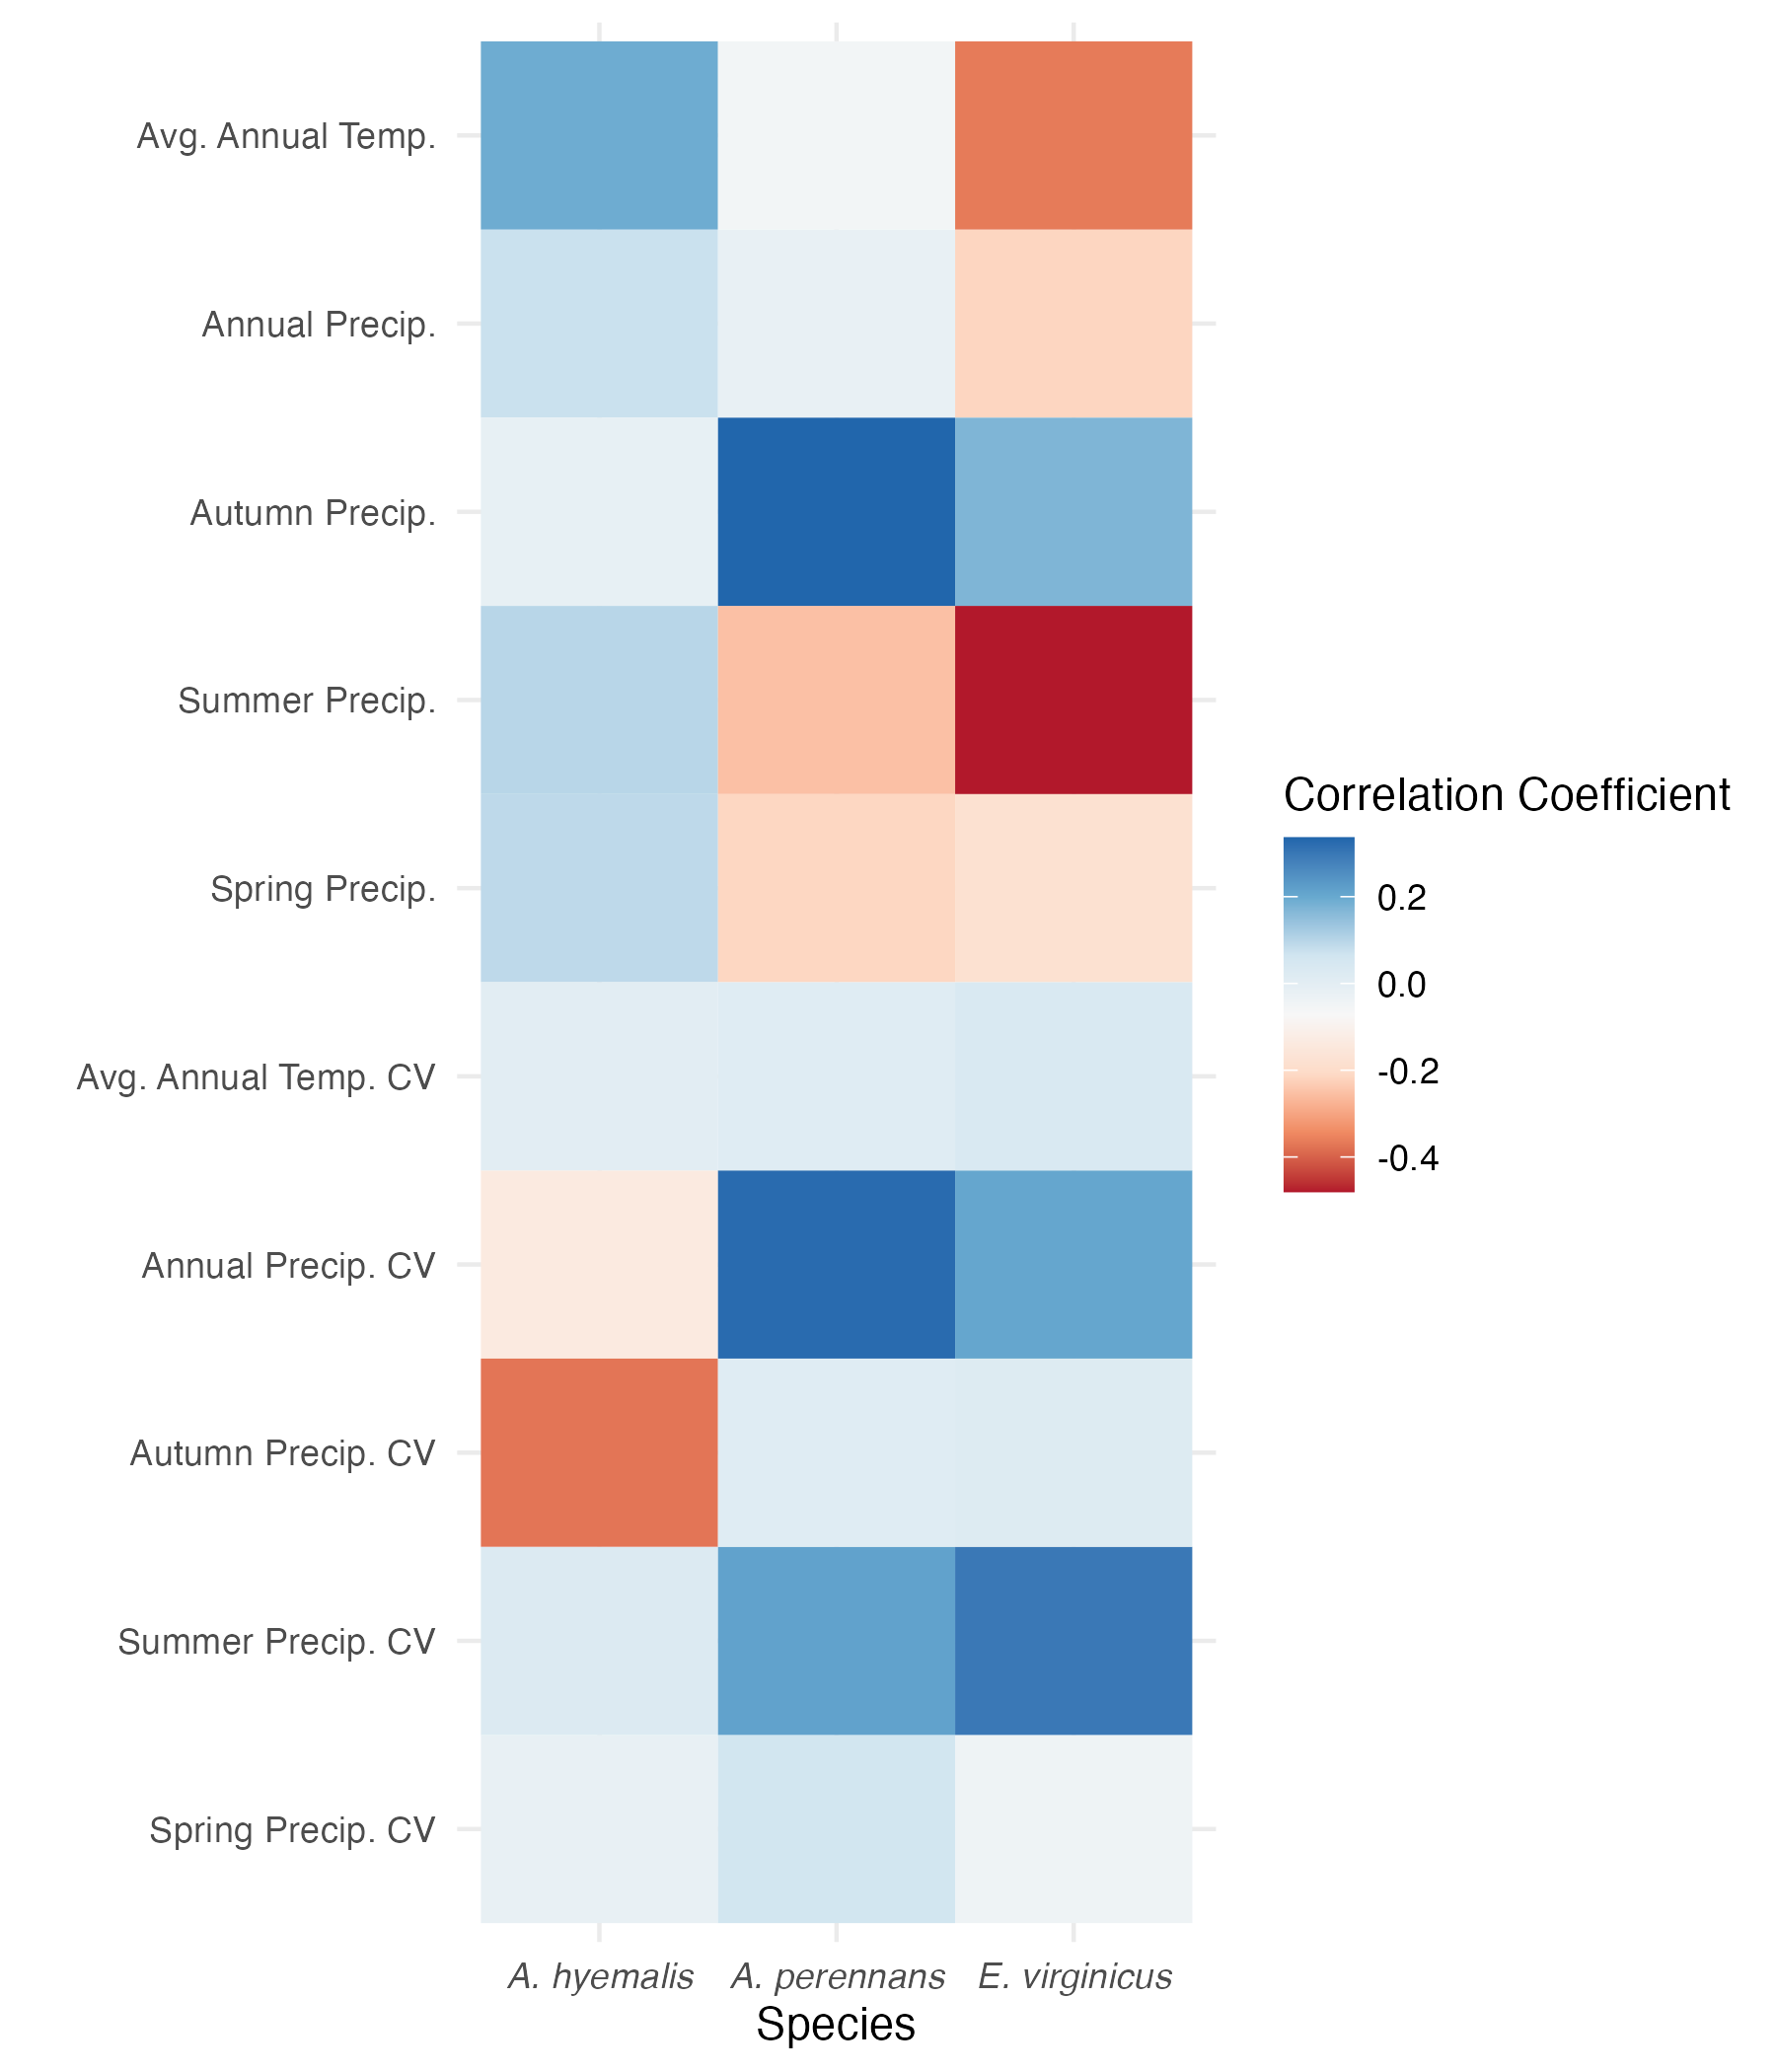
\includegraphics[width = .8\linewidth]{climate_corr_heatmap.png}
	\caption{\textbf{Changes in climate drivers associated with relative change in endophyte prevalence.} Color denotes the Pearson correlation coefficient between the relative rate of change in endophyte prevalence and the change in annual mean temperature ($^oC$) and cumulative seasonal precipitation (mm), as well as the change in coefficient of variation of each climate driver.}
\end{figure}

\section*{Discussion}
Our examination of historic plant specimens revealed a cryptic biotic reponse to climate change. 
The geographic distributions and phenology of macroorganisms are apparent indicators of climate change.
For the three host species we examined, there have been clear increases in fungal endophyte prevalence over the last two centuries.
This increase suggests that \emph{Epichloë} fungal endophytes are playing key adaptive roles in response to climate change and that the mutualism between grasses and their fungal endophytes has contributed to resilience for each partner species under the observed changes in climate. 
Spatial and temporal trends in endophyte prevalence varied between each species in ecologically meaningful ways.
Our spatially-explicit model predicted regions of both high and low endophyte prevalence, suggesting that symbiotic and non-symbiotic host plants have overlapping, but non-identical niche requirements. 
Endophytes may expand the range of their hosts by allowing them to persist in environments where they otherwise could not \citep{afkhami2014mutualist, kazenel2015mutualistic}.
Understanding how microbial symbionts respond to climate change is a first step towards incorporating reciprocal host-symbiont interactions into predictions host range shifts.


For \emph{E. virginicus}, we found greater increases in prevalence in regions that have become drier during the Summer, the species' peak growing season. 
Fitness benefits of the symbiosis under drought conditions could explain this increase and also explain high predicted prevalence towards the species' northern range edge coinciding with a strong latitudinal decline in precipitation. 
Previous population surveys for endophytes in this species found similar latitudinal trends in prevalence \citep{sneck2017variation,rudgers2009benefits}, but at smaller scales. 
Following previous work demonstrating drought benefits in a greenhouse manipulation with \emph{A. hyemalis} \citep{davitt2011understanding}, we had predicted  that endophyte prevalence should similarly increase at a greater rate in regions that have seen reduced precipitation, yet we found the opposite trend in our herbarium surveys and that changes in prevalence for this species had the weakest correlations with climate drivers.
Given that the study region has experienced relatively moderate changes in precipation and in temperature, potentially the magnitude of climate change has not been great enough to cause larger changes in endophyte prevalence for this species. 
Weak associations with drought could also be explained by climate-driven changes in the rate of imperfect transmission (the generation of non-symbiotic offspring from symbiotic hosts), which could counterbalance endophyte-mediated fitness benefits, and leading to stable intermediate prevalence rates \citep{donald2021context}. 
To our knowledge, the response of the symbiosis in \emph{A. perennans} to drought has not been examined experimentally, but in a separate greenhouse experiment, endophytes had a positive effect on reproduction under shaded, low-light conditions \citep{davitt2010costs}. 
\emph{Epichloë} endophytes have been connected to a suite of non-drought related fitness benefits including herbivore protection \citep{brem2001epichloe}, salinity resistence \citep{wang2020effects}, and mediation of the soil microbiome \citep{roberts2015rhizosphere}, potentially mediated by the diverse bioactive alkaloids and other signaling compounds they produce \citep{saikkonen2013chemical}.
The strong increase in symbiotic \emph{A. perennans} could be explained by these diverse benefits. 
Differences between the responses of each species underscore that while all of these C3 grasses share similar broad-scale distributions, each engages in unique biotic interactions and has unique niche requirements.

Our analysis advances the use of herbarium specimens in two ways. 
First and foremost, this is the first study to link long-term changes in microbial symbioses to changes in climate using specimens from natural history collections.
The responses of microbial symbioses are a rich target for future studies within museum specimens, particularly those that take advantage of advances in sequencing technology.
While we used relatively coarse presence/absence data based on fungal morphology, other studies have examined historic plant microbiomes using molecular sequencing and sophisticated bioinformatics techniques, but these studies have so far been limited to relatively few specimens at limited spatial extents \cite{yoshida2015computational, heberling2019utilizing, bieker2020metagenomic, gross2021hidden, bradshaw2021global}. 
Continued advances in capturing historic DNA and in filtering out potential contamination during specimen storage \citep{daru2019novel, bakker2020herbarium, raxworthy2021mining} will be imperative in the effort to scale up these efforts. 
This scaling up will be essential to be able to quantify changes not just in the prevalence of symbionts, but also in symbionts' intraspecific variation and evolutionary responses to climate change, as well as  in changes in the wider microbial community. 
Answering these questions as well as the unknown questions that future researchers may ask also reiterates the value in capturing meta-information during ongoing digitization efforts at herbaria around the world and during the accession of newly collected specimens \citep{lendemer2020extended}.
Second, we accounted for several potential biases in the data observation process that may be common to many collections-based research questions by using a spatially-explicit random effects model. 
Spatial autocorrelation \cite{willems2022forest}, potential biases introduced by the sampling habits of collectors \citep{daru2018widespread}, and variation between contemporary researchers during the collection of trait data, if not corrected for could lead to biased inference about the strength and direction of historic change.
Fitting this model in a Bayesian framework allows for full propagation of uncertainty.

Ultimately, a central goal of global change biology is to generate predictive insights into the future of natural systems. 
While this survey of historic endophyte prevalence is necessarily correlative, it serves as a foundation to develop better predictive models of the response of microbial symbioses to climate change. 
Combining the insights from this sort of regional-scale survey with field experiments and physiological data could be invaluable. 
While we found that climate is strongly correlated with endophytes' temporal responses, we do not know why trends in prevalence were weak in some areas or how endophytes would respond to more extreme changes in climate.
For example, transplanting symbiotic and non-symbiotic plants beyond the range edge of \emph{A. hyemalis} could tell us whether persistent lack of endophytes in that area is a result of environmental conditions that lead the symbiosis to negative fitness consequences, or is a result of some historical contingency or dispersal limitation that has thus far limited the presence of symbiotic hosts from a region where they would otherwise flourish and provide resilience.
While we observed evidence of mutualism resilience, more extreme environmental changes than those observed in our study could potentially push one or both partners beyond their physiological limit, leading to the collapse of the mutualism. 
Our analysis thus far is agnostic to changes in the distributions of hosts. 
Mechanistic models could connect the responses of both host and symbionts to abiotic climate drivers integrating dispersal processes. 
Beyond host-microbe symbioses, building these types of models would work towards quantitatively attributing biotic responses to anthropogenically driven climate change, similar to methods in climate science and economics \citep{stott2010detection, carleton2016social}.
%Elymus genotype
%Agrostis weedy



	%%%%%%%%%%%%%%%%%%%%%
	% Acknowledgments
	%%%%%%%%%%%%%%%%%%%%%
	% You may wish to remove the Acknowledgments section while your paper 
	% is under review (unless you wish to waive your anonymity under
	% double-blind review) if the Acknowledgments reveal your identity.
	% If you remove this section, you will need to add it back in to your
	% final files after acceptance.
	
	\section*{Acknowledgments}
	We thank Jessica Budke for help in drafting our initial destructive sampling plan, and to the many members of herbarium staff who facilitated our research visits, as well as to the hundreds of collectors who contributed to the natural history collections. 
	This research was supported by funding from NSF grant () and from funding from the Texas Ecolab Program.


	%%%%%%%%%%%%%%%%%%%%%
	% Statement of Authorship
	%%%%%%%%%%%%%%%%%%%%%
	% This section should also be commented out while your MS is undergoing
	% double-blind review. The specifics should of course be adapted to
	% your paper, but the paragraph below gives some hints of possible
	% contributions.
	
	\section*{Statement of Authorship}
	

	
	\section*{Data and Code Availability}
	
	On initial submission, you may use this section to provide a URL for editors and reviewers that is `private for peer review'. After acceptance, this section must be updated with correct, working DOIs for data deposits (typically on the Dryad Digital Repository, \citealt{CookEtAl2015}) and code deposits (such as in Zenodo). 
	
	\section*{Appendix A: Additional Methods and Parameters}
	\renewcommand{\thefigure}{A\arabic{figure}}
	\setcounter{figure}{0}
	
		\renewcommand{\thetable}{A\arabic{table}}
	\setcounter{equation}{0}  % reset counter 
	\setcounter{figure}{0}
	\setcounter{table}{0}
	
	\begin{figure}[H]
		\centering
		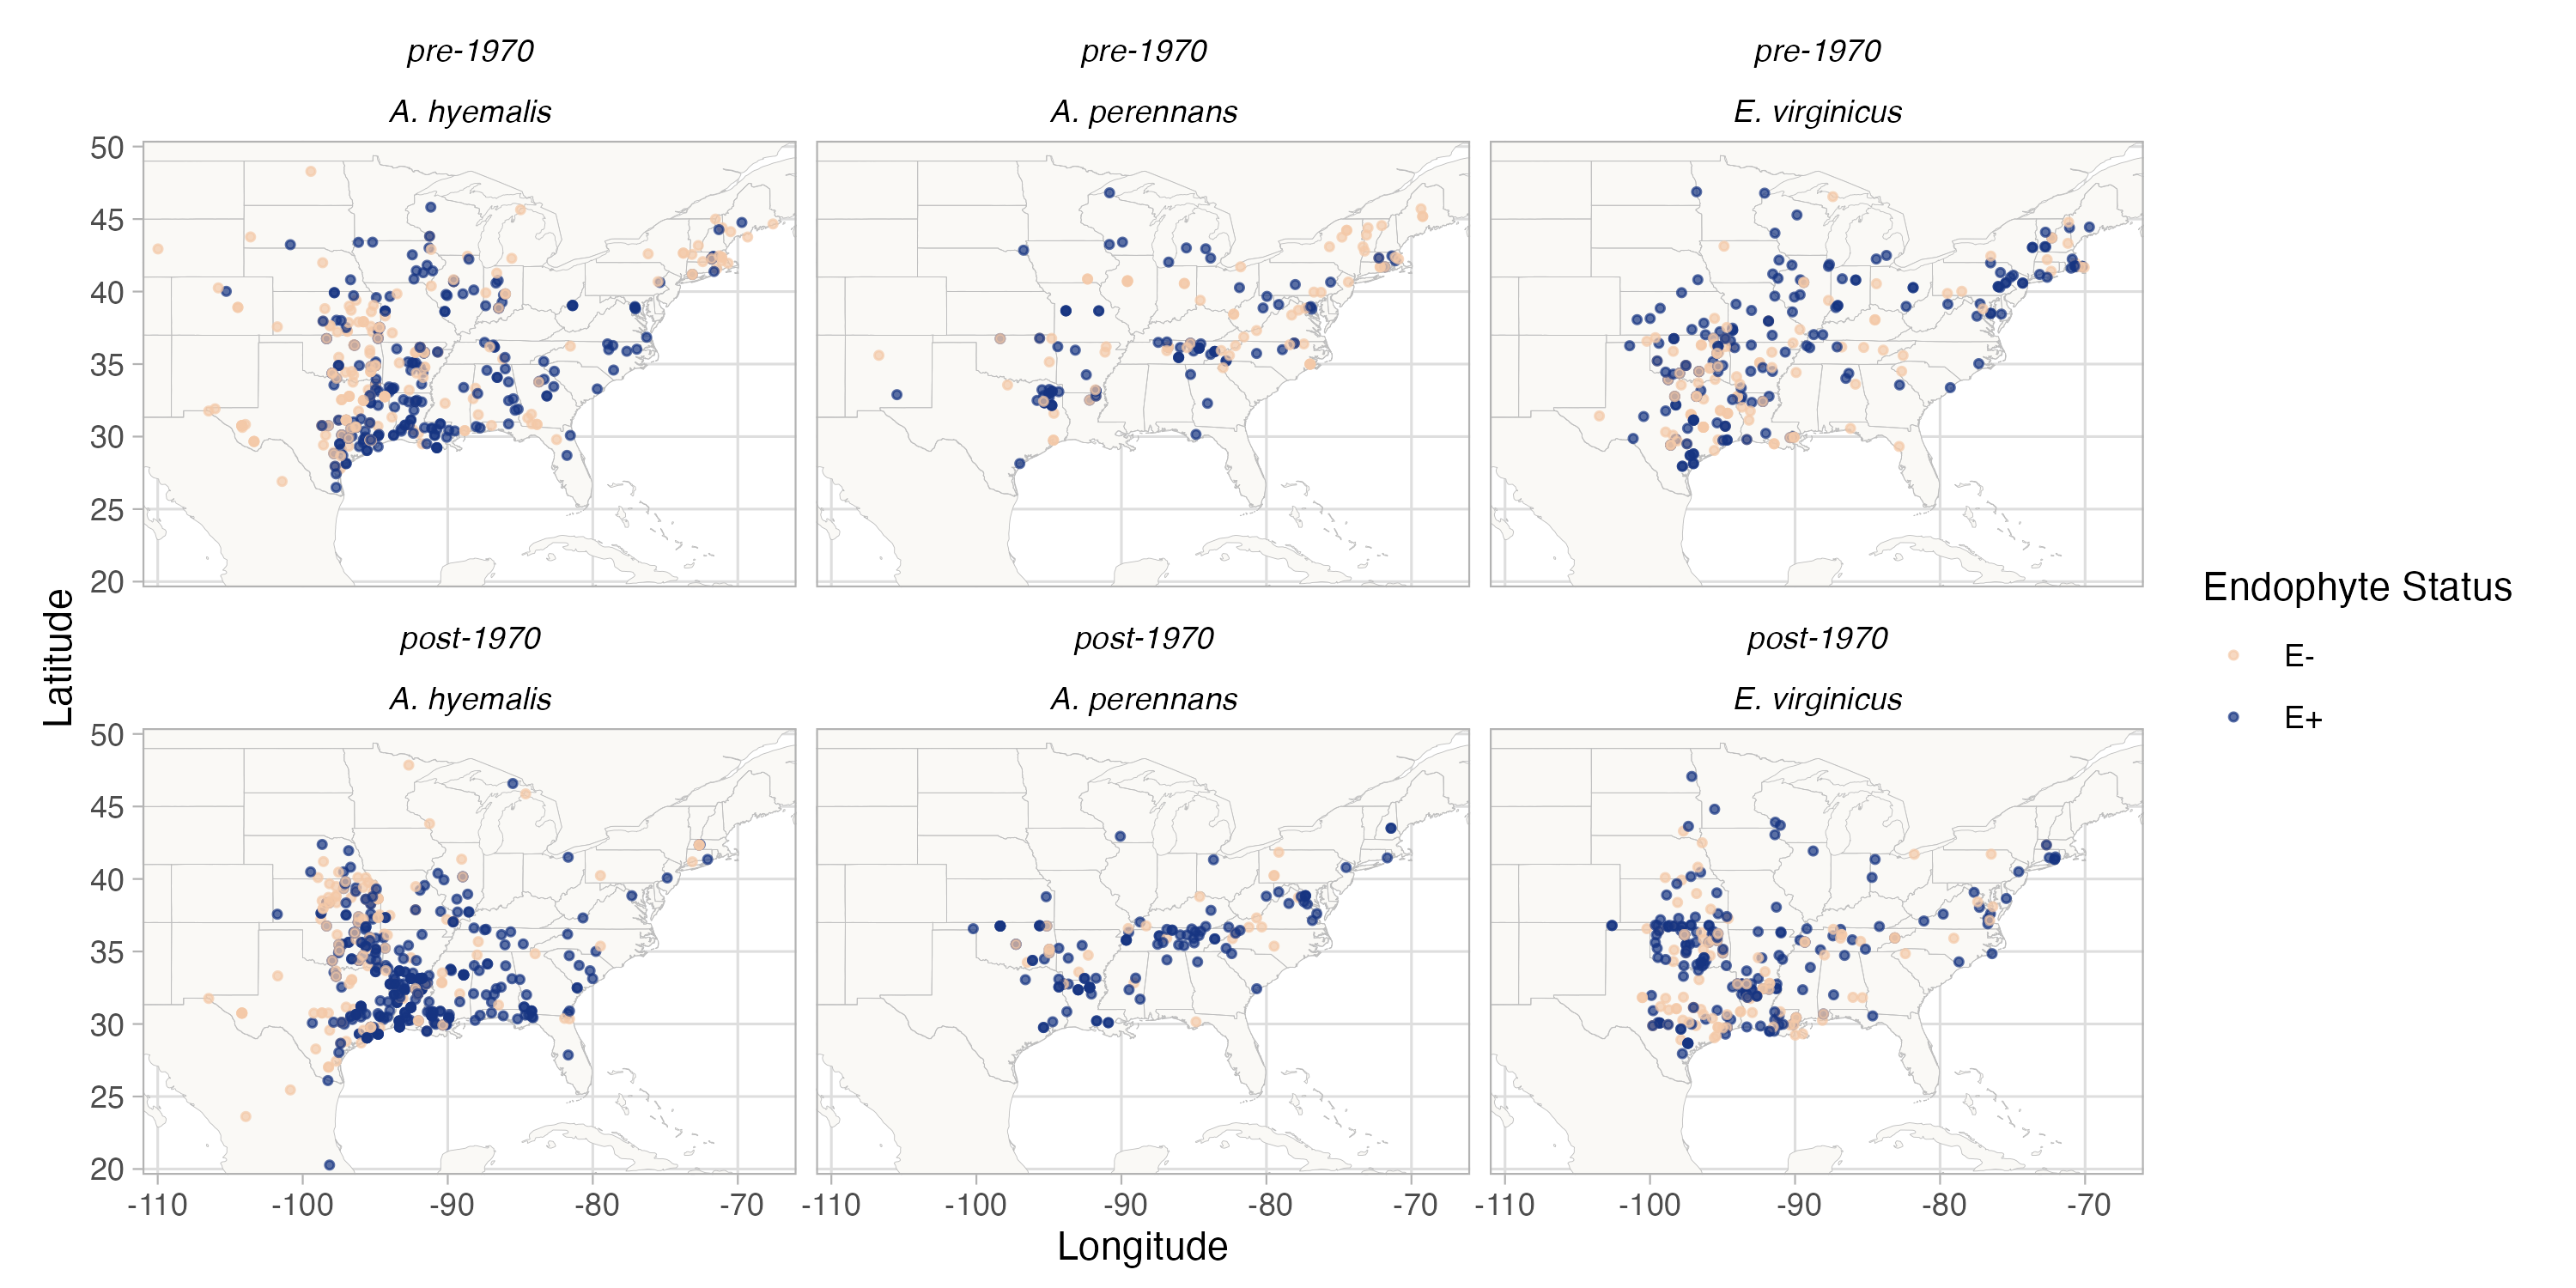
\includegraphics[width = \linewidth]{endo_status_map.png}
		\caption{\textbf{Endophyte presence/absence in specimens of each host species.} Points show collection locations colored according to whether the specimen contained endophytes ( E+; blue points) or did not contain endophytes (E-, tan points) and are faceted based on collection period.}
	\end{figure}
	
	\begin{figure}[H]
		\centering
		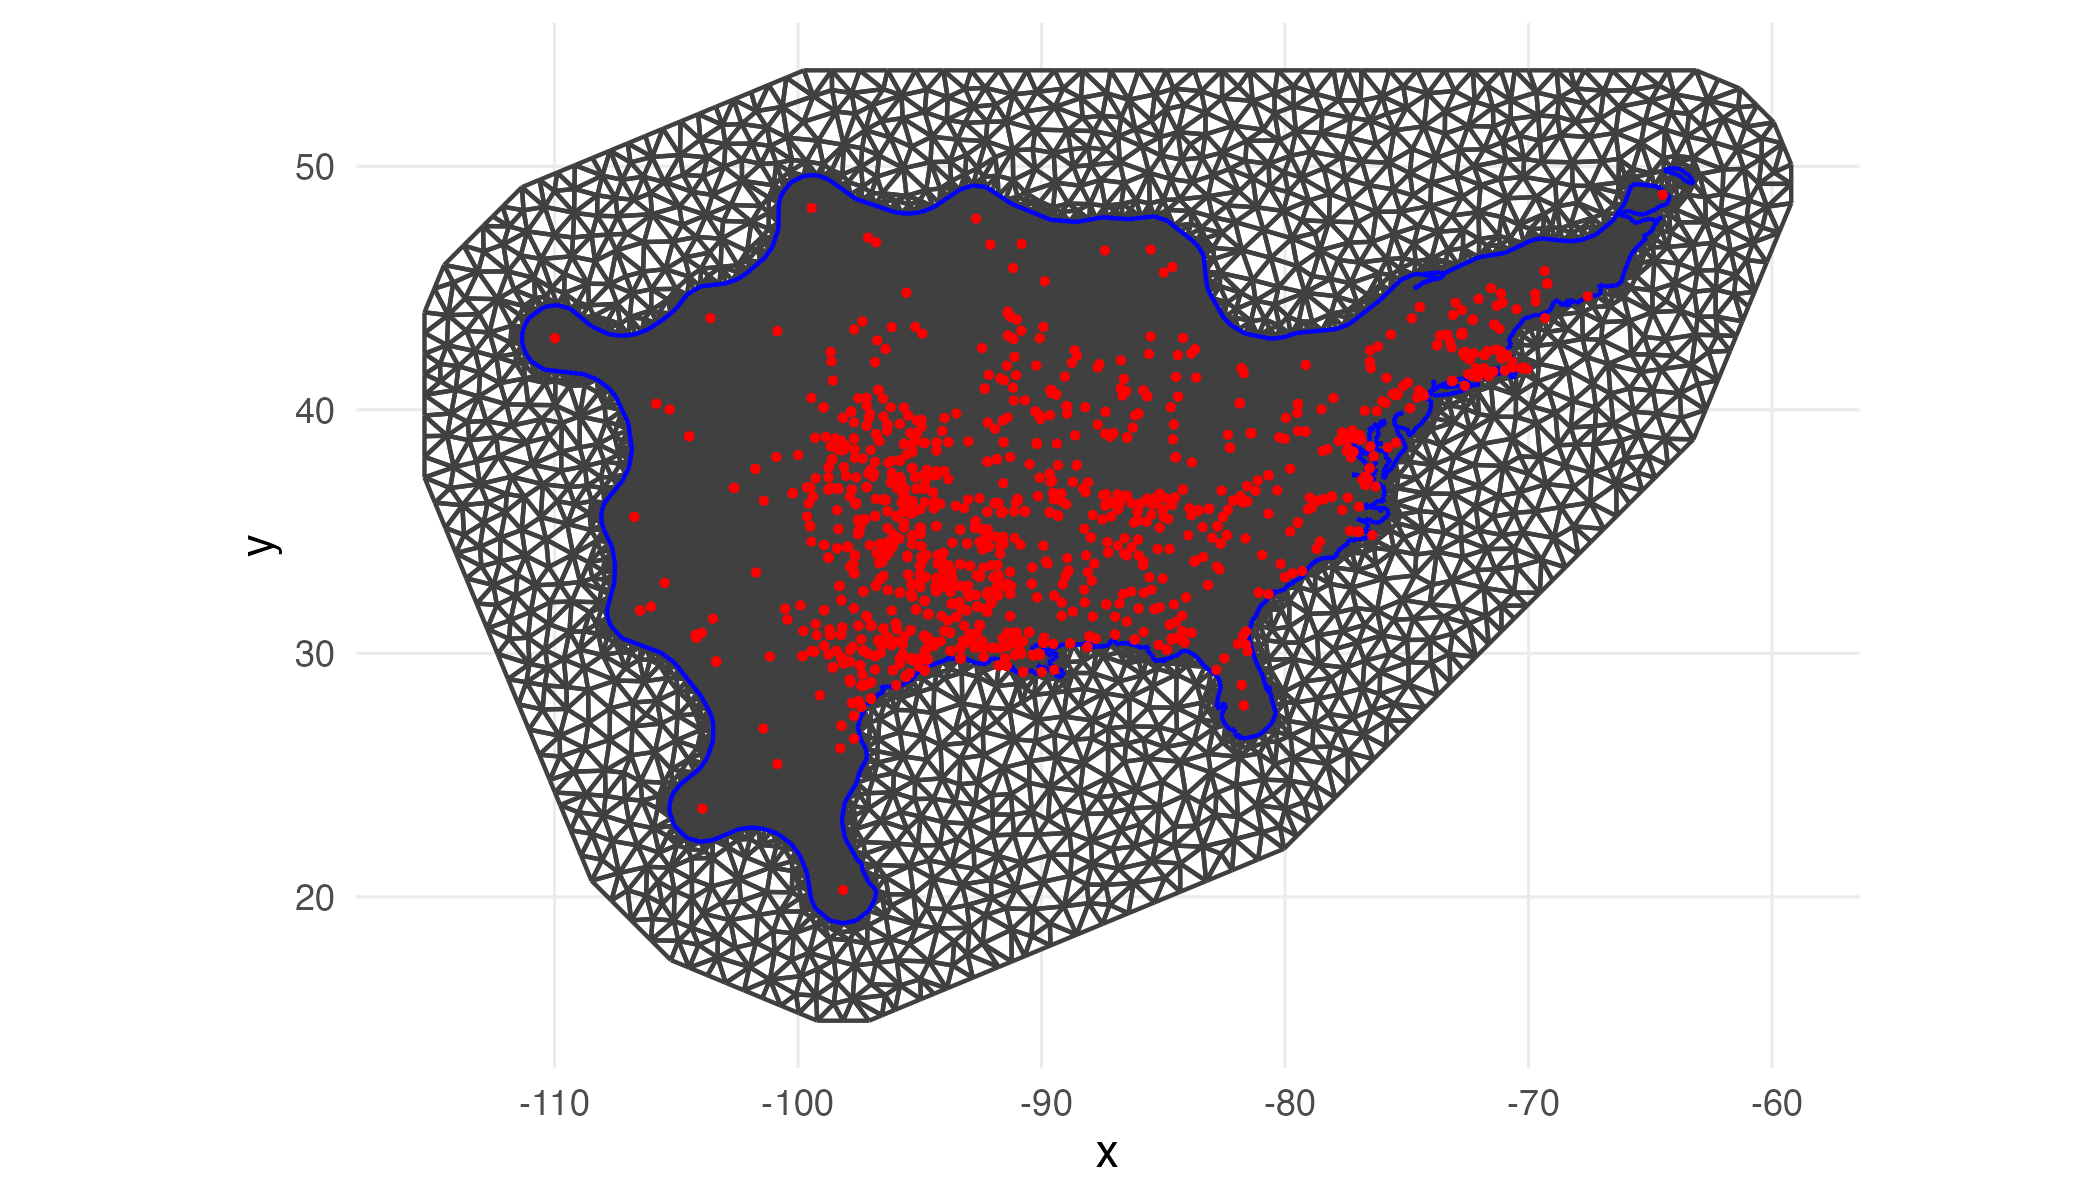
\includegraphics[width = \linewidth]{mesh_plot.png}
		\caption{\textbf{Delauney triangulation mesh used to estimate spatial dependence between data points}. Grey lines indicate edges of triangles used to define distances between observations. Red points indicate locations of sampled herbarium specimens, and the blue outlines show the international borders used to define the edge of the mesh along coastlines.}
	\end{figure}

\begin{figure}[H]
	\centering
	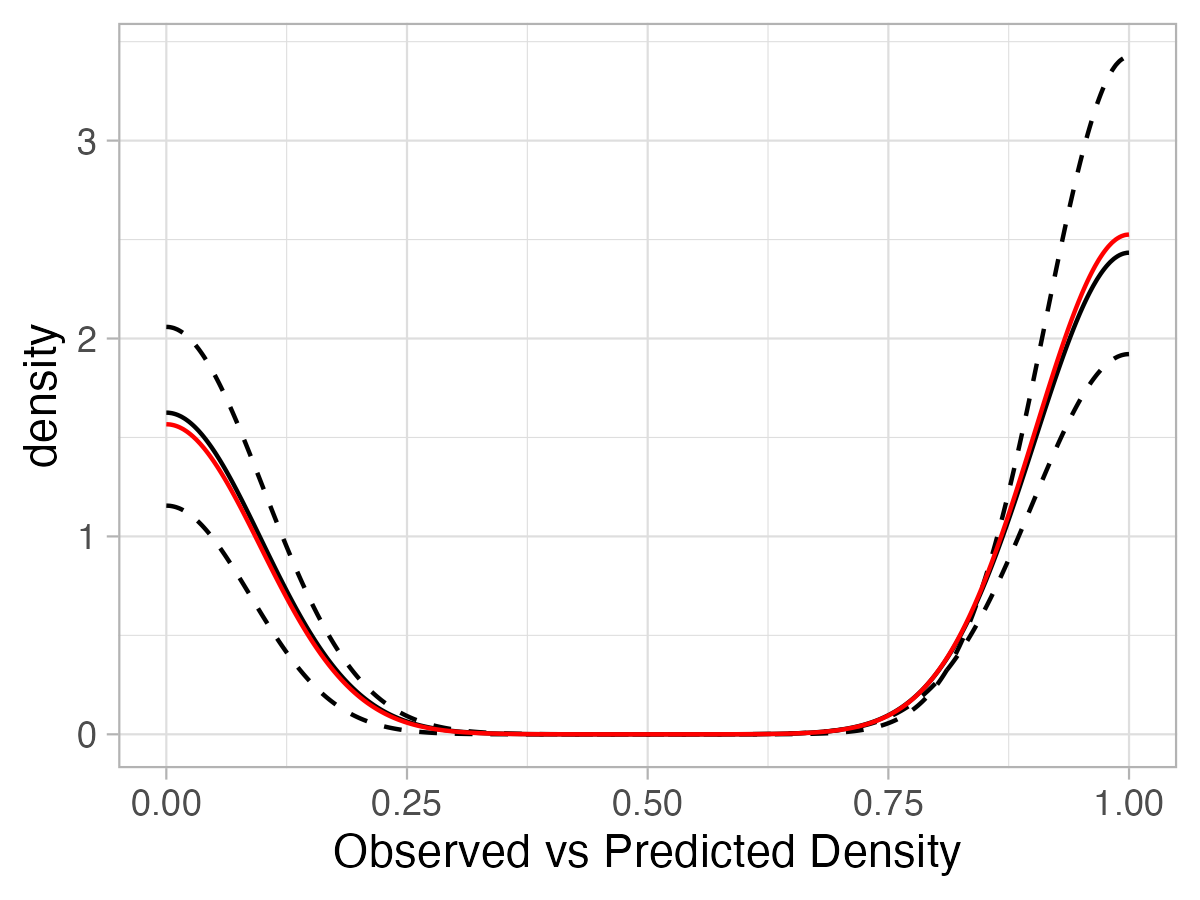
\includegraphics[width = .8\linewidth]{density_plot.png}
	\caption{\textbf{Consistency between real data and simulated values indicate that the fitted model accurately describes the data}. Graph shows density curves for the observed data (red) along with the mean(solid) and 95\% CI (dashed) of simulated values (black).}
\end{figure}

	
	\begin{figure}[H]
		\centering
		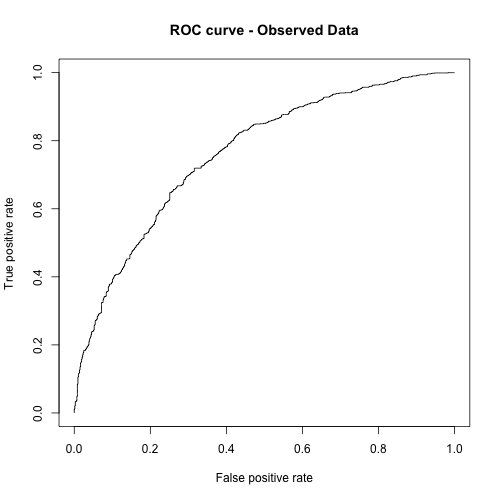
\includegraphics[width = .5\linewidth]{ROC_plot.png}
		\caption{\textbf{ROC plot showing model performance classifying observations according to endophyte status.} The curves show adequate model performance for observed (top) and test (bottom) data. The AUC for each is 0.77 and 0.81 respectively.}
	\end{figure}

	\begin{figure}[H]
	\centering
	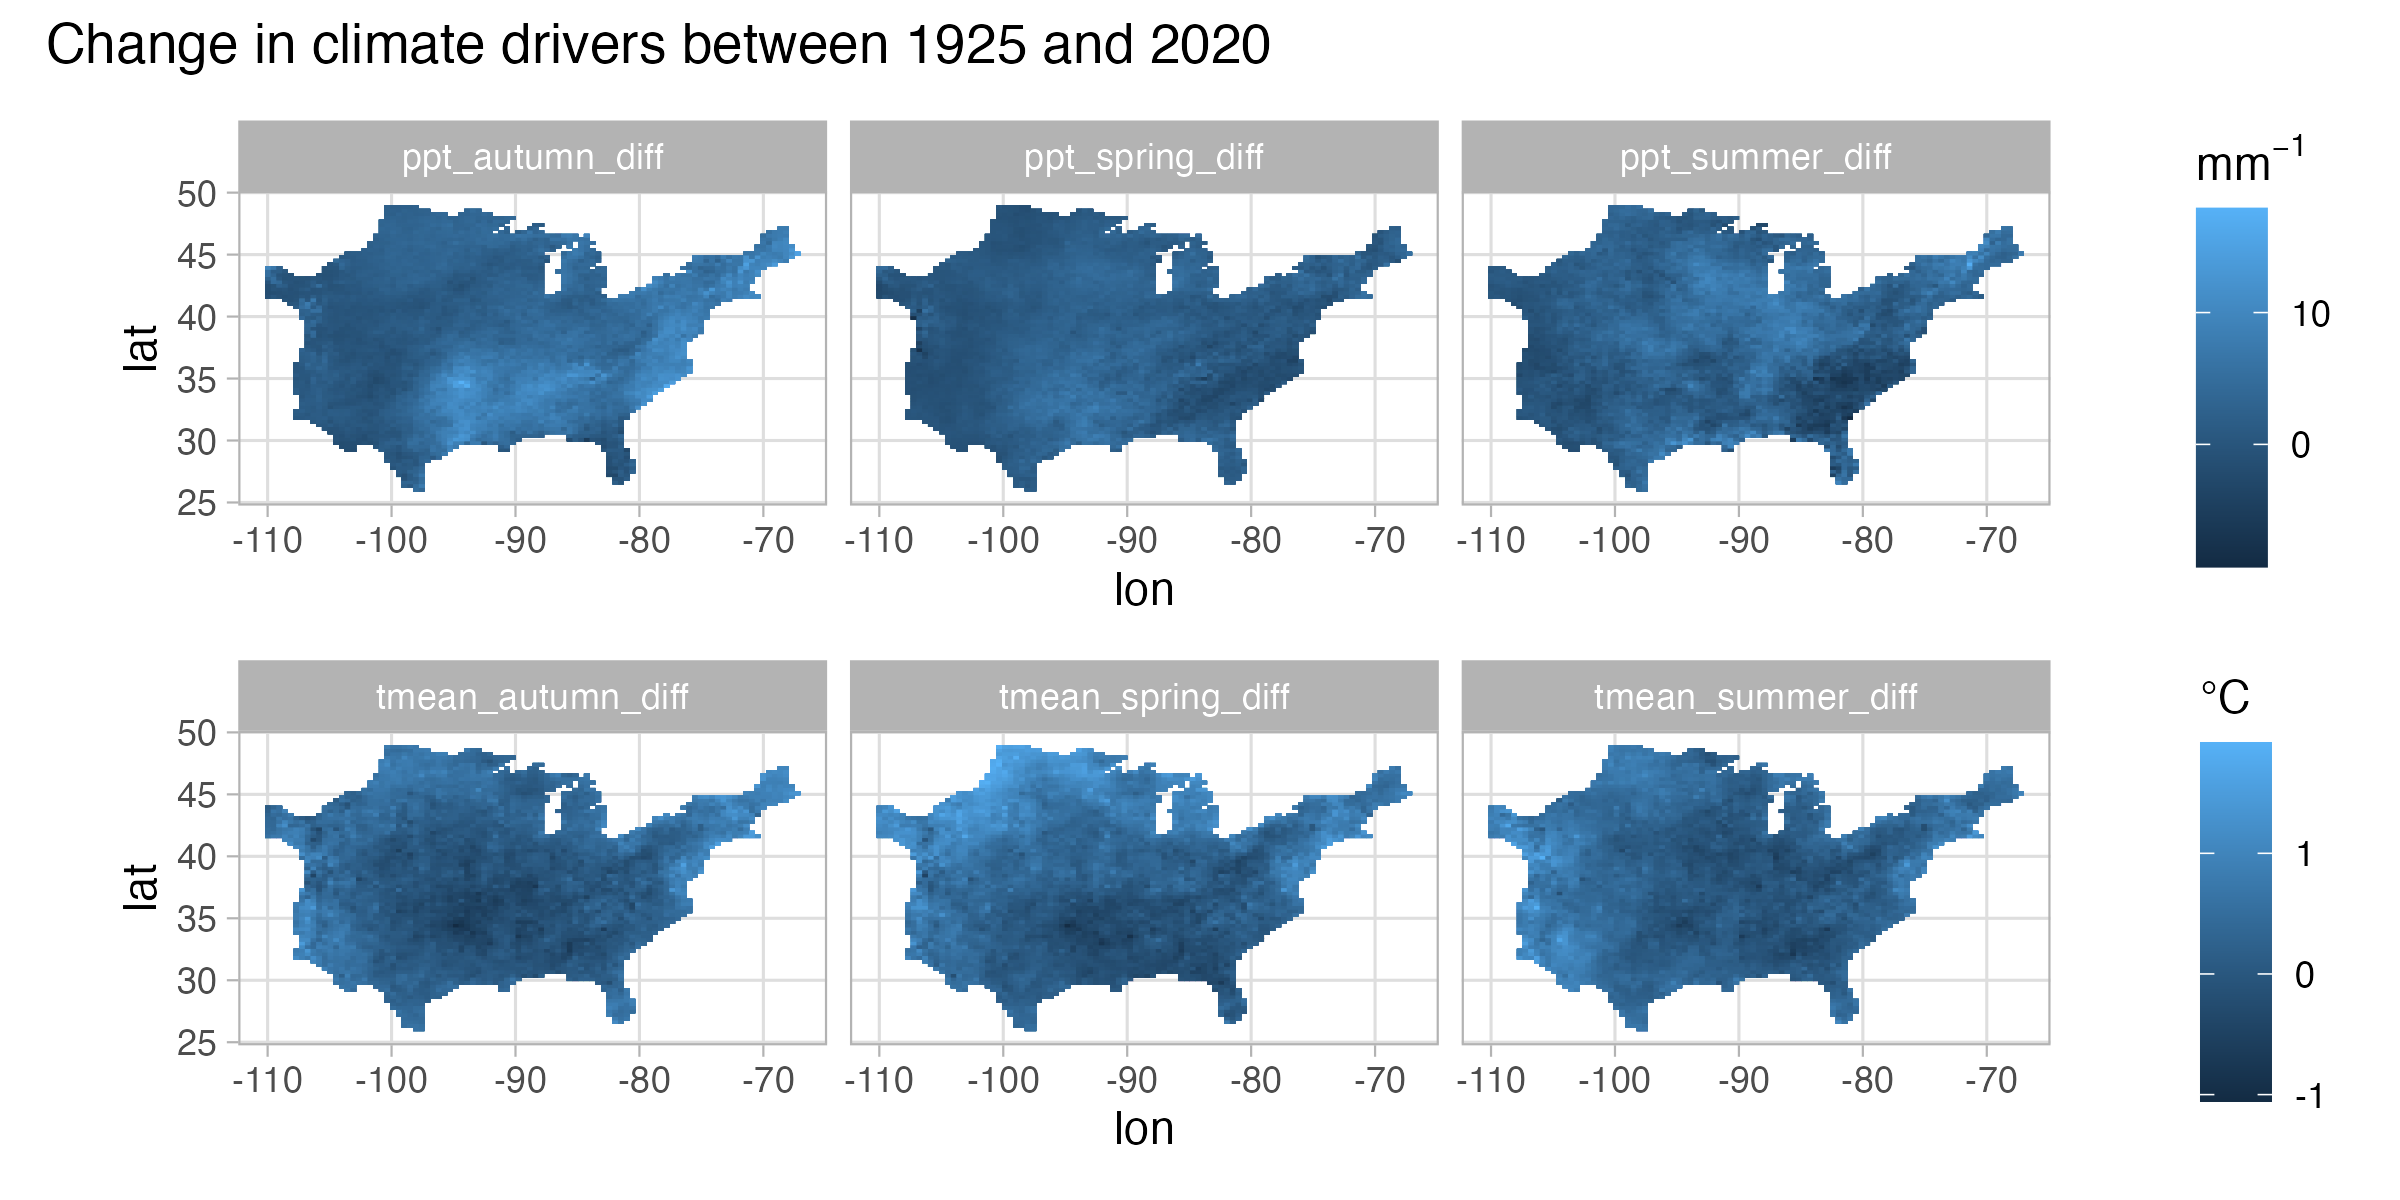
\includegraphics[width = \linewidth]{climate_change_plot.png}
	\caption{\textbf{Change in 30-year climate normals between the periods ending in 1915 and 2020.} Color represented change in cumulative precipitation (top row) and average seasonal temperature (bottom row) for the study area.}
\end{figure}

	
	
	\begin{table}[h]
		\caption{Summary of herbarium sampling}
		\label{Table:herbaria}
		\centering
		\begin{tabular}{llll}\hline
			Collection        & AGHY        & AGPE      &      ELVI\\ \hline
			Botanical Research Institute of Texas &      &    &        \\
			Louisiana State University &       &   &          \\
			Mercer Botanic Garden &       &      &     \\
			Missouri Botanic Garden&  & & \\
		    Texas A\&M &  & & \\
		    University of Kansas &  &&  \\
		    University of Oklahoma &  &&  \\
		    University of Texas     &  & & \\		    				 			     			     
			Oklahoma State University&       &       &   \\ \hline
		\end{tabular}
		\bigskip{}

	\end{table}
	
	
	
	
	% In most cases, authors should typeset supplementary material in a separate,
	% author-supplied PDF. For author-supplied PDFs, please consult the
	% AmNat_supp_template.tex document, available from
	% https://www.journals.uchicago.edu/journals/an/instruct 
	%
	% By contrast, the Appendix instructions below apply to cases in which
	% a brief appendix is to appear in print after the main body of the article.
	% That notably includes descriptions of methods, tables defining parameters,
	% and other material necessary for reproducing the MS's results.
	%
	% Please reset counters for the appendix (thus normally figure A1, 
	% figure A2, table A1, etc.).
	%
	% Most AmNat articles have no more than one print appendix. If your article
	% has more than one, counters for each appendix should match the letter of
	% that appendix. For example, tables in Appendix B should be numbered table B1, % table C2, etc. This applies to tables, equations, and figures.
	%
	% It's better not to use the \appendix command, because we have some
	% formatting peculiarities that \appendix conflicts with.
	
	%%%%%%%%%%%%%%%%%%%%%
	% Bibliography
	%%%%%%%%%%%%%%%%%%%%%
	% You can either type your references following the examples below, or
	% compile your BiBTeX database and paste the contents of your .bbl file
	% here. The amnatnat.bst style file should work for this---but please
	% let us know if you run into any hitches with it!
	%
	% If you upload a .bib file with your submission, please upload the .bbl
	% file as well; this will be required for typesetting.
	%
	% The list below includes sample journal articles, book chapters, and
	% Dryad references.
\bibliographystyle{plain}
\bibliography{endo_herbarium}
	
	\newpage{}
	

	
\end{document}

